\section{Diogenes in a nutshell}

In this section we show the main features of our tools.
%
Firstly, we give an overview of possible \coco processes
that you can write within Eclipse. 
Then, we present the verification tool for java programs.

The plugin supports the full \coco syntax and you can check
the honesty of any valid process (if decidable); however,
only a subset of processes can be translated to a java program, 
so the following examples are limited to this subset.

\paragraph{Contracts}
A contract describes the intended behaviour of \emph{one} of the two
participants involved in a session.  We use binary session
types~\cite{Honda98esop} to define contracts.  Session types are terms
of a process algebra featuring internal/external choice, and
recursion.

Suppose we are modelling a store: it waits for receive
an \atom{order}, then it answers \atom{amount} or \atom{abort}.
The answer depends on another service, \ie an insurance service,
which waits for a \atom{req}est, then it responds \atom{ok} or \atom{no}.

The two contracts can be written as follows:
%
\begin{lstlisting}[language=coco,basicstyle=\scriptsize\ttfamily]
contract C { order? string . ( amount! int (+) abort! ) }
contract D { req! string . ( ok? + no? ) }
\end{lstlisting}
External actions are followed by the question mark (\code{?}) and grouped
with the symbols \code{+}; similarly we use the
exclamation mark (\code{!}) and the symbol \code{(+)} for
internal actions and choices.

The corresponding java contract is
\begin{mdframed}
\begin{minted}[
    fontsize=\scriptsize
    %,linenos
    ]{java}
ContractDefinition C = def("C").setContract(
    externalSum()
    .add("order", Sort.string(), 
        internalSum()
        .add("amount", Sort.integer())
        .add("abort", Sort.unit())));
        
ContractDefinition D = def("D").setContract(
    internalSum()
    .add("req", Sort.string(), 
        externalSum()
        .add("ok", Sort.unit())
        .add("no", Sort.unit())));
\end{minted}
\end{mdframed}
where \code{def()}, \code{externalSum()}, \code{internalSum()} 
are static methods of a factory.

\paragraph{Specification}
A possible specification of a contract-oriented service is
\begin{lstlisting}[
    language=coco,
    basicstyle=\scriptsize\ttfamily,
    numbers=left,
    numbersep=12pt]
specification Pdishonest {
    tellAndWait x C .
    receive x [
        order? v:string . (
            tellAndWait y D . (
                send y req! v .
                receive y [
                    ok? . send x amount! 100
                    + no? . send x abort!
                    + t . send x abort!]))]
}
\end{lstlisting}

The contract \code{C} is published at line \lineno{2} and the store waits
until the session starts.
Once the session $x$ is established, the store waits
to receive an \atom{order}, 
binding it to the variable $v$ (lines \lineno{3} and \lineno{4}).
Then, the store advertises the contract \code{D}, waits to establish a session
$y$ (line \lineno{5}) and send a \atom{req}uest (\lineno{6}) passing 
the value $v$.
Finally, it waits to receive a response \atom{ok} or \atom{no},
and responds \atom{amount} or \atom{abort} on $x$. 
\inlineCoco{t} models a timeout that covers the case of no response (lines \lineno{7},
\lineno{8}, \lineno{9} and \lineno{10}).

The above specification is \emph{dishonest}. If the session $y$
is never fused, the store is stuck in $x$ and cannot fulfil the contract \code{C}.
Furthermore, what happens if the a response arrive after the timeout?

A possible solution can be:
\begin{lstlisting}[
    language=coco,
    basicstyle=\scriptsize\ttfamily,
    numbers=left,
    numbersep=12pt]
specification Phonest {
    tellAndWait x C .
    receive x [
        order? v:string . (
            tellRetract y D . (
                send y req! v .
                receive y [
                    ok? . send x amount! 100
                    + no? . send x abort!
                    + t . (send x abort! | receive y [ok? + no?])]) 
            : send x abort!)]
}
\end{lstlisting}
In line \lineno{5} we use the \inlineCoco{tellRetract}: if the contract \code{D}
is not fused in time, the contract is retracted and the control pass to line \lineno{11}.
Finally we can change the timeout \inlineCoco{t} behaviour, adding a parallel
execution of a \inlineCoco{receive} \emph{without timeout}.

The specification does not aim to be completed. On refining the implementation,
the user must provide suitable timeout values, and 
the order's amount should be derived in some way.

\hidden{
The \cref{fig:outline} shows the outline derived from the above specification.

\begin{figure}[H]
\centering
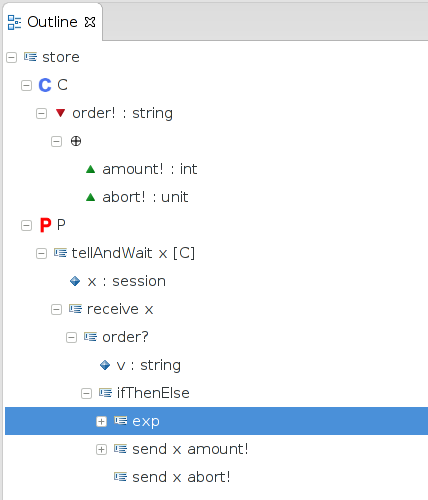
\includegraphics[scale=0.4]{img/outline.png}
\label{fig:outline}
\caption{caption}
\end{figure}
}

\paragraph{Code generation}
The plugin automatically generates corresponding Maude and Java files.
The former can be used directly within Eclipse to verify its honesty,
exploiting the model-checking tool of~\cite{verifiable};
the latter represents a working java skeleton. 
Considering the honest specification describe above, the skeleton looks like
\begin{mdframed}
\begin{minted}[
    fontsize=\scriptsize
    ,linenos
    ]{java}
public class Phonest extends Participant {
            
    public void run() {
        Session<TST> x = tellAndWait(C);    
        Message msg = x.waitForReceive("order");
        
        String v;
        v = msg.getStringValue();
        
        Public<TST> pbl_y = tell(D, 10000);
        try {
            Session<TST> y = pbl_y.waitForSession();
            y.sendIfAllowed("req", v);
            
            try {
                Message msg_1 = y.waitForReceive(10000, "ok", "no");
                
                switch (msg_1.getLabel()) {                    
                    case "ok": x.sendIfAllowed("amount", 100); break;
                    case "no": x.sendIfAllowed("abort"); break;                    
                }
            }
            catch (TimeExpiredException e) {
                parallel(()->{ x.sendIfAllowed("abort"); });
                parallel(()->{ y.waitForReceive("ok", "no"); });
            }            
        }
        catch(ContractExpiredException e) {
            x.sendIfAllowed("abort");
        }
    }
}
\end{minted}
\end{mdframed}

The \inlineCoco{tellRetract} corresponds to perform a tell with
a delay (line \lineno{10}). The successive \code{waitForSession()} blocks until the delay is
expired, throwing a \code{ContractExpiredException} if the session 
was not fused in time (the contract has been retracted).
The timeout \inlineCoco{t} corresponds to a \code{waitForReceived} with a timeout.
The method blocks until a message with label \code{"ok"} or \code{"no"} is received,
or throws a \code{TimeExpiredException} if the timeout expires.


\paragraph{Honesty verification}
Diogenes allows to verify the honesty of Java programs. 
The only constrains that have to be respected are
\begin{itemize}
\item extends the 
\end{itemize}

